\newpage
\section{Алгоритмы кластеризации}

\subsection{Виды расстояний}
\subsubsection{Между объектами}
{\it Для начала давайте разберёмся, как лучше всего выбирать расстояние между объектами?}

Вариантов выбора способа задания расстояния огромное множество, но мы будем рассматривать только некоторые, наиболее популярные, из них.
\begin{enumerate}
\item Минковского
\[
d_r({\bf x, y}) = \left( \sum\limits_{j=1}^{N} |x_j - y_j|^r \right)^{\frac{1}{r}}
\]
\item Евклидово $(r = 2)$
\[
d_{E} ({\bf x, y}) = d_2({\bf x, y})
\]
\item Манхеттен $(r = 1)$ "--- расстояние, которое надо пройти пешеходу.
\[
d_{M} ({\bf x, y}) = d_1({\bf x, y})
\]
\item $r = \infty$
\[
d_{\infty} ({\bf x, y}) = \max\limits_{j} |x_j - y_j|
\]
\item Жаккар
\[
d_{J} ({\bf x, y}) = 1 - \frac{|x_j \cap y_j|}{|x_j \cup y_j|}
\]
\item Косинус
\[
d_{C} ({\bf x, y}) =\arccos\frac{{\bf xy}}{||{\bf x}|| \cdot ||{\bf y}||}
\]
\item Правки\\
$d_{e}$ "--- наименьшее количество удалений и вставок, приводящее {\bf x} к {\bf y};
\item Хэмминг\\
$d_{H}$ "--- количество различных компонент в {\bf x} и {\bf y}.

\end{enumerate}


\subsubsection{Между кластерами}
А теперь предположим, что мы уже разбили наши объекты, на какое-то количество кластеров и хотим определить, на каком расстоянии кластеры расположены друг относительно друга.
Для этого используются следующие способы задания расстояния:
\begin{enumerate}
\item Single-linkage
\[
d_{\min} (C_i,C_j) = \min\limits_{{\bf x} \in C_i, {\bf y} \in C_j} ||{\bf x} - {\bf y}||
\]
\item Complete-linkage
\[
d_{\max} (C_i,C_j) = \max\limits_{{\bf x} \in C_i, {\bf y} \in C_j} ||{\bf x} - {\bf y}||
\]
\item Average
\[
d_{avg} (C_i,C_j) = \frac{1}{n_j n_i} \sum\limits_{{\bf x} \in C_i}  \sum\limits_{{\bf y} \in C_j} ||{\bf x} - {\bf y}||
\]
\item Mean
\[
d_{mean} (C_i,C_j) = ||{\bf m_i} - {\bf m_j}||
\]
\end{enumerate}
\newpage
\subsection{Иерархическая кластеризация}
\subsubsection{Идея метода}

Мы все из биологии помним, что всё живое на земле делится на следующую иерархию: царство, порядок, семейство, род, вид и так далее. Каждая из ступенек этой иерархии является непересекающейся группой, которую мы и будем называть кластером.

{\bf Суть} иерархической кластеризации заключается в том, чтобы взять и разделить весь наш {\it input space} (входное пространство) на части, но только не плоско, а, грубо говоря, вложено. То есть снача мы делим на несколько частей, каждая из которых делится ещё и ещё до тех пор, пока результат нас не устроит. 

Есть 2 достаточно очевидных, но принципиально разных способа реализации данного алгоритма "--- {\it Agglomerative} (восходящие) и {\it Divisive} (нисходящие).

Визуализация данных, как правило, осуществляется с помощью {\bf дендрограммы} (дерево, то есть граф без циклов).

\subsubsection{Agglomerative}
Наиболее подходит для случая, когда нам нужно получить большое количество кластеров.
Так же данный вариант обычно немножко проще реализуется.
\begin{enumerate}
\item начинаем с ситуации, когда каждый объект – отдельный кластер;
\item на каждом шаге совмещаем два наиболее близких кластера, получая из них один новый;
\item останавливаемся, когда получаем требуемое количество или единственный кластер.
\end{enumerate}

\begin{figure}[H]
\centering
    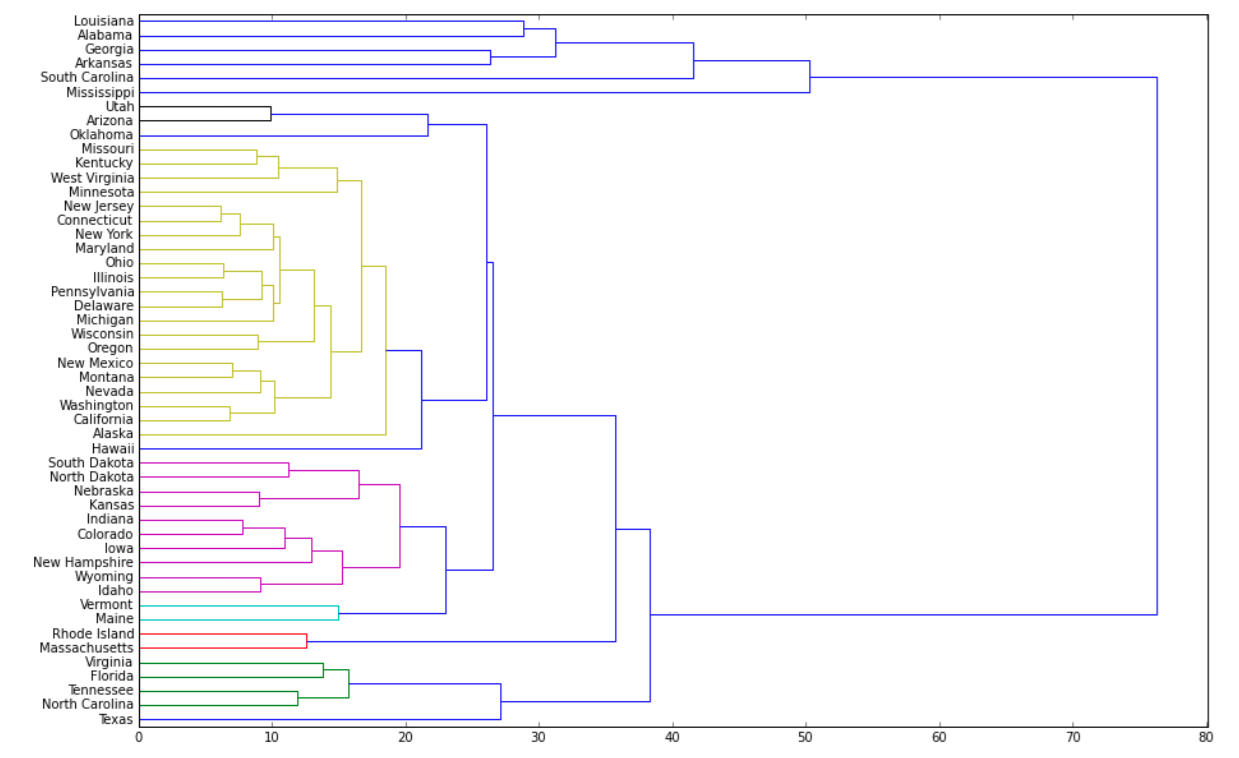
\includegraphics[width=150mm]{images/agl.png}
    \caption{Пример дендограммы восходящей кластеризации на основе красно-синих штатов.}
    \label{alg}
\end{figure}

\subsubsection{Divisive}
Более удобен, когда нам нужно несколько кластеров.
\begin{enumerate}
\item начинаем с ситуации, когда все объекты составляют один большой кластер;
\item на каждом шаге разделяем каждый кластер две или несколько частей;
\item останавливаемся, когда получаем требуемое количество или заранее заданное $N$ кластеров.
\end{enumerate}

\begin{figure}[H]
\centering
    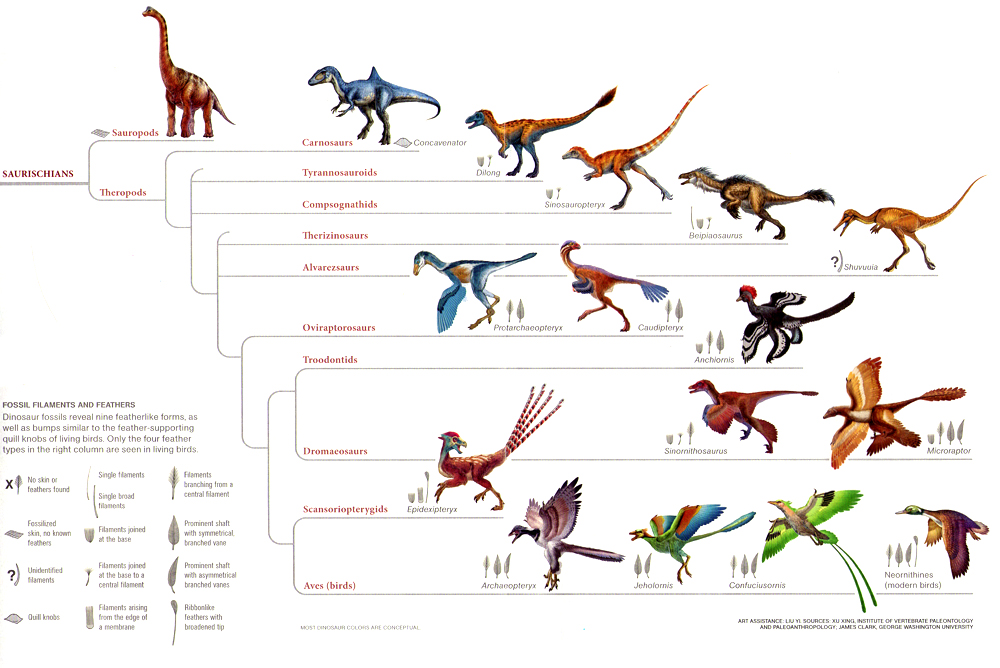
\includegraphics[width=150mm]{images/dino.jpg}
    \caption{Пример дендограммы нисходящей кластеризации на основе классификации динозавров.}
    \label{dino}
\end{figure}


\subsubsection{Реализация алгоритма}
Рассмотрим восходящий алгоритм в виде псевдокода на языке $Python$:
\begin{lstlisting}
function agglomerative(X, K):
    initialize N # number of objects 
    initialize C = N # number of clusters initialize 
    C_i = x_i # initial clusters 
    while C>K:
        C_a = C_b = None # closest clusters 
        min_dist = +inf # distance between closest 
        for i in 1 .. C:
            for j in i + 1 .. C:
                dist = d(C_i, C_j) # dist. betw. clusters 
                if dist < min_dist:
                    min_dist = dist 
                    C_a = C_i 
                    C_b = C_j
        merge(C_a, C_b)
        C=C - 1
    return C_1, ... , C_k
\end{lstlisting}

Как мы видим, необходимая память $O(N^2)$, а вычислительная сложность данного алгоритма $О(N^2 \log N)$ (хорошо, что не куб). Получается, что этот алгоритм вычислительно очень дорогой и применять его на очень больших объемах данных очень непродуктивно, и никакой памяти не хватит. Но у него есть несколько приемуществ: удобная визуализация и не сложно выбрать количество кластеров.

\subsubsection{Stepwise-optimal HC}
Что плохого в том алгоритме, что мы описали выше?

На каждом шаге мы пытаемся совместить два кластера, но не очень понимаем почему и зачем. Понятно, что минимальное расстояние между класстерами -- это хорошо. Придумали сделать некое обобщение этого алгоритма, который позволяет делать всё тоже самое для произвольного критерия качества ($J$).

Окаывается, что те расстояния между кластерами, которые мы использовали, имеют под собой функционал, который они оптимизируют. В частности 
$d_{max}$ обеспечивает наименьшее увеличение диаметра кластера.
Так же часто используется расстояние
$d_e$ (см.~\ref{de}), которое обеспечивает наименьшее увеличение квадратичного критерия (квадратичный критерий "--- это сумма расстояний внутри кластера от каждого объекта, до соответствующего центра).

\begin{equation}\label{de}
d_e(C_i,C_j) = \sqrt{\frac{n_i n_j}{n_i+n_j}}||m_i - m_j||
\end{equation}

Рассмотрим данный алгоритм в виде псевдокода на языке $Python$:
\begin{lstlisting}
function swo(X, K):
    initialize N # number of objects
    initialize C = N # number of clusters initialize 
    C_i = x_i # initial clusters 
    while C > K:
        # choose the pair that optimizes
        # the given criterion J when merged
        C_a, C_b = find_best_merge(J, C_1, ..., C_C) 
        merge(C_a, C_b)
        C=C - 1
    return C_1, ... , C_k
\end{lstlisting}

\subsubsection{Неевклидовы пространства}

{\it Как измерить расстояние между кластерами, если невозможно определить центроид?}

Оказывается, что иерархический подход так же работает, но только нужно изменить функцию растояния между кластерами.

{\bf Идея.} В каждом из кластеров выбрать <<типичныи представителя>> "–-- clustroid. Считать расстояние не между кластерами, а между <<кластроидами>>

Каким образом выбрать <<типичного представителя>> ?

Есть несколько подходов. 
Можно выбать такой объект, для которого
\begin{itemize}
\item минимальная сумма расстояний до других объектов в кластере (он находится в центре);
\item сумма квадратов расстояний до других объектов в кластере минимальна; 
\item максимальное расстояние до других объектов в кластере минимально.
\end{itemize}

Таким образом можно кластеризовать что-то другое помимо числовых векторов.

\subsubsection{Плюсы и минусы алгоритма}
\begin{itemize}
\item[+] Могут получиться несферические кластеры;
\item[+] Можно придумать разнообразие критерии, как разнообразные виды расстояния между кластерами, так и между объектами;
\item[+] Поддерживает любые $K$ из коробки (то есть один раз запустив алгоритм, мы уже кластеризовали наши объекты на любое количество кластеров);
\item[-] Требует много вычислительных ресурсов, невозможно работать при больших объёмов данных.
\end{itemize}

\subsection{<<Быстрая>> модификация алгоритма}
\begin{lstlisting}
function fast_agglomerative(X, K):
    initialize N # number of objects
    initialize C = N # number of clusters initialize 
    C_i = x_i # initial clusters initialize 
    delta_set = get_delta_set(C_i) 
    while C > K:
        C_a = C_b = None # closest clusters 
        min_dist = +inf # distance between closest 
        for C_i in delta_set:
            for C_j in delta_set:
                dist = d(C_i, C_j) # dist. betw. clusters 
                if dist < min_dist:
                    min_dist = dist
                    C_a = C_i; C_b = C_j 
        new_cluster = merge(C_a, C_b)
        update_delta_set(C_i, new_cluster) 
        C = C - 1
        if delta_set is empty:
            delta_set = get_delta_set(C_i) 
    return C_1, ..., C_K
\end{lstlisting}

{\it Осталось только понять, что же такое этот delta-set и откуда его брать.}

{\bf Delta-set} --– набор кластеров расстояние между которыми меньше $\delta$. Чтобы реализовать функцию {\bf get-delta-set} нужно учитывать следующие моменты:
\begin{enumerate}
\item Если $C \le K_1$, то $\delta$-set – это все $C_i$;
\item Иначе выбрать $K_2$ случайных расстояний между кластерами, $\delta = \min{K_1,K_2}$;
\item $K_1$ и $K_2$ влияют только на скорость, но не на результат кластеризации; 
\item рекомендованные значения $K_1 = K_2 = 20$.
\end{enumerate}
\newpage

\subsection{DBSCAN}
DBSCAN "--- {\it <<Density Based Spatial Clustering of Applications with Noise>>} (плотностный алгоритм для кластеризации пространственных данных с присутствием шума) впервые был предложен Мартином Эстер, Гансом-Питером Кригель и их коллегами в 1996 году как решение проблемы разбиения (изначально пространственных) данных на кластеры произвольной формы.

Основная {\bf идея} алгоритма заключается в том, что внутри каждого кластера наблюдается {\it типичная плотность точек} (объектов), которая заметно выше, чем плотность вне этого кластера. Также есть области {\it шума}, плотность которых згачительно меньше плотности любого из кластеров. Дабы отделить шум от основных класстеров задаётся некоторое значение, соответствующее минимальному пороговому значению точек в кластере, а~именно {\it Min\_Pts}

А теперь для удобства рассуждений введём несколько определений.

\begin{Def}{Плотность} 
"--- количество объектов внутри сферы заданного радиуса $\e$.
\end{Def}
\begin{Def}{Core-объект} \label{core}
"--- объект, плотность вокруг котрого больше, чем  Min\_Pts.
\end{Def}
\begin{Def}{Граничный объект} 
"--- объект, плотность вокруг котрого меньше, чем  Min\_Pts, однако он находится в непосредственной близости с Core-объектом.
\end{Def}
\begin{Def}{Шум} 
"--- объект, который не является ни core-объектом, ни граничным объектом. 
\end{Def}
\begin{Def}{Кластеры}
"--- участки высокой плотности, состоящие из core-объектов и граничных-объектов, разделенные участками низкой плотности.
\end{Def}

Таким образом, для реализации алгоритма нам понадобиться два параметра: $\e$ и {\it Min\_Pts}.

\subsubsection{Алгоритм}
На вход подаём множество объектов --- $X$, $\e$-радиус <<соседства>> и минимальное количество объектов в~кластере $Min\_Pts$. Рассмотрим алгоритм в виде псевдокода на языке $Python$:
\begin{lstlisting}
def DBSCAN(X, eps, Min_Pts):
    initialize NV = X # not visited objects
    for x in NV:
        remove(NV, x) # mark as visited
        nbr = neighbours(x, eps) # set of neighbours
        if nbr.size < Min_Pts:
            mark_as_noise(x)
        else:
            C = new_cluster()
            expand_cluster(x, nbr, C, eps, min_pts, NV)
    return C

def expand_cluster(x, nbr, C, eps, min_pts, NV):
    add(x, C)
    for x1 in nbr:
        if x1 in NV: # object not visited
            remove(NV, x1) # mark as visited
            nbr1 = neighbours(x1, eps)
            if nbr1.size >= min_pts:
                # join sets of neighbours
                merge(nbr, nbr_1)
        if x1 not in any cluster:
            add(x1, C)
\end{lstlisting}

\subsubsection{Плюсы и минусы}
\begin{itemize}
\item[$+$] не требуется заранее знать количество кластеров;
\item[$+$] кластеры могут быть произвольной формы. К тому же может случиться такое, что один кластер будет полностью лежать в другом, но они не будут соприкасаться;
\item[$+$] в данном алгоритме присутствует понятие шума, поэтому он устойчив к выбросам;
\item[$+$] для работы алгоритмы достаточно всего два параметра.
\end{itemize}
\begin{itemize}
\item[$-$] не является вполне детерминированным, так как если граничные точки равноудалены сразу от двух кластеров, то они могут быть быть интерпретированными по разному в зависимости от порядка обхода множества объектов;
\item[$-$] не работает при большой разности в плотностях кластеров, потому что нельзя подобрать комбинацию $\e$ и {\it Min\_Pts} соответствующим образом сразу для всех кластеров;
\item[$-$] если нет чёткого понимания природы данных, с которыми предстоит работать, то бывает трудно подобрать параметры $\e$ и {\it Min\_Pts}.
\end{itemize}

\subsubsection{Вычислительная сложность}
В общем случае алгоритм DBSCAN имеет квадратичную вычислительную сложность ({\bf $n^2$}) за счёт поиска $\e$-соседства. Однако, если для этой цели использовать специальную структуру данных "--- $R*Tree$, то в результате сложность поиска $\e$-соседей для одной точки – $O(\log n)$. Таким образом общая вычислительная сложность алгоритма DBSCAN составляет {\bf $O(n \log n)$}.

\subsubsection{Пример}
Зафиксируем параметры $\e = \frac{\sqrt{13}}{2} + \delta$ (расстояние между точками B1 и B2 + некое маленькое $\delta > 0$) и~$Min\_Pts = 3$. В случае~(\ref{DBSCAN1}) в качестве стартовой точки выберем B1, а в случае~(\ref{DBSCAN2}) "--- B2. Несложно заметить, что результаты полчатся разные. 
В первом случае B2 "--- граничная точка для кластера B, 
а во втором "--- шум.
\begin{figure}[H]
\centering
    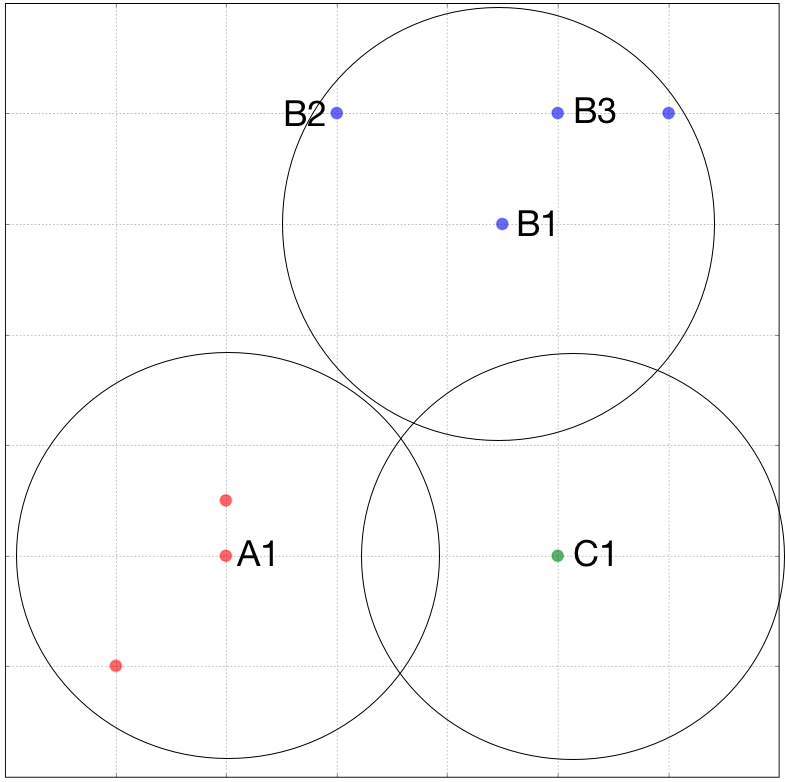
\includegraphics[width=60mm]{images/DBSCAN1.png}
    \caption{Пример кластеризации методом DBSCAN с начальной точкой B1.}
    \label{DBSCAN1}
\end{figure}
\begin{figure}[H]
\centering
    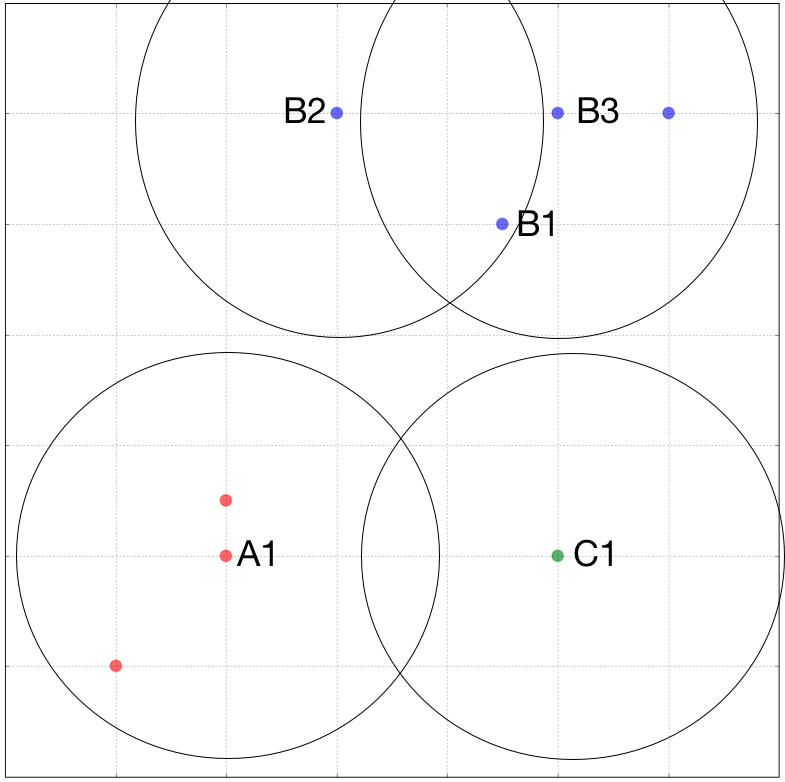
\includegraphics[width=60mm]{images/DBSCAN2.png}
    \caption{Пример кластеризации методом DBSCAN с начальной точкой B2.}
    \label{DBSCAN2}
\end{figure}


\subsection{Оценка качества алгоритма кластеризации}
{\it Вот предположим, что у нас есть какие-то данные, есть готовая кластеризация, но нам этого мало. Мы~сели и ручками написали свой алгоритм кластеризации. Как можно оценить качество нашего алгоритма?}

Пусть нам заведомо дана обучающая выборка, для которой правильная кластеризация $C$ известна. С помощью выбранного алгоритма получена кластеризация K и проверим, насколько K совпадает с C. Для этого используем такие понятия, как {\it Adjusted Rand Index} (ARI) и {\it Mutual Information} (MI)
\[
RI = \frac{a+b}{C^N_2}, \qquad ARI = \frac{RI - E_{rdm}[RI]}{\max(RI) - E_{rdm}[RI]},
\]
где $a$ "--- количество пар объектов, попавших в один кластер и в C, и в K,\\
а $b$ "--- кол-во пар объектов, попавших в разные кластеры и в C, и в K.
\[
MI = \sum\limits_{c \in C}\sum\limits_{c \in K} p(c,k) \log \frac{p(c,k)}{p(k)p(c)}.
\]


{\it А что делать, если изначально <<правильной>> кластеризации попросту нет в наличии?!} {\it И как выбирать параметры нашей для нашей кластеризации?!}

\subsubsection{Критерий Silhouette (<<силуэт>>)}
Пусть дана кластеризация $N$ объектов в $K$ кластеров, и в каждом кластере $C_k$ находтся $N_k$ объектов. Предположим, что~наш объект i попал в $C_k$, тогда
\begin{itemize}
\item a(i) "--- среднее расстояние от i объекта до объектов из его же кластера $C_k$:
\[
a(i) = \frac{1}{N_{k} - 1} \sum\limits_{j \in C_k } d_k(i,j),
\]
где $d_k(i,j)$ "--- расстояние между $i$ и $j$ объектами; 
\item $b(i) = \min\limits_{j \not= k} b_{j}(i)$, где $b_{j}(i)$ "--- минимальное среднее расстояние от i объекта до объектов из другого кластера $C_j$ (то есть расстояние до соседнего кластера, куда бы он мог попасть, если бы не в этот кластер).
\end{itemize}
Таким образом
\[
silhouette(i) = S_i = \frac{b(i) - a(i)}{\max \left(a(i),b(i)\right)} 
\]
Заметим, что если наша кластеризация хорошая, то $b(i)$  всегда будет больше, чем $a(i)$, и $\max(a(i),b(i)) = b(i)$.
А оценкой качества нашего алгоритма будет являться средний {\it silhouette} для всех точек из множества {\bf X.} То есть
\[
SWC = \frac{1}{N} \sum\limits_{j = 1}^{N} S_j.
\]
То значение $K$, для которого $SWC$ будет максимально, выбирается в качестве оптимального количества кластеров.
\begin{Zam}
Если $K$ окажется равным $1$, то $SWC = -1$.
\end{Zam}
\subsection{OPTICS}
OPTICS "--- {\it <<ordering points to identify the clustering structure>>. }


{\bf Основная идея} "--- не ограничиваться фиксированной плотностью, как в DBSCAN, а варьировать ее в зависимости от того, как много объектов попадают в $\e$-окрестность.

Как в алгоритме DBSCAN, OPTICS требует двух параметров: $\e$, который описывает максимальное расстояние (радиус) для оценки плотности, и $MinPts$ "--- та самая минимальная плотность, то есть количество объектов, необходимых для формирования кластера. 
Однакое, в отличии от DBSCAN, OPTICS также учитывает то, что точки могут являться частью более плотного кластера, поэтому вводится понятие $core\_distance$, которое описывает расстояние до ближайшей точки внутри круга радиуса $MinPts$.
\[
core\_distance(p) = 
\begin{cases}
\mathrm{UNDEFINED},\quad \text{if } |N_{\e} (p)| < MinPts;\\
\text{{\it MinPts} is the smallest distance to } N_{\e}(p), \quad \mathrm{otherwise}.
\end{cases}
\]

Так же введём понятие $reachability\_distance$, описывающее расстояние от объекта $O$ до $p$ или $core\_distance(p)$:
\[
reachability\_distance(p) = 
\begin{cases}
\mathrm{UNDEFINED},\quad \text{if } |N_{\e} (p)| < MinPts;\\
\max(core\_dist(p),dist(p,O)), \quad \mathrm{otherwise}.
\end{cases}
\]

Если окажется так, что $O$ и $P$ "--- ближайшие друг к другу объекты, то необходимо, что бы в конечном итоге они оказались в одном кластере.

Оба <<новых>> параметра будут неопределены, если в районе данной точки не будет распологаться достаточно плотный кластер, удовлетворяющий основным параметрам ($\e, MinPts$).

\subsubsection{Алгоритм OPTICS}

Рассмотрим данный алгоритм в виде псевдокода на языке $Python$:
\begin{lstlisting}
function optics(X, eps, min_pts)
    for each point x in X:
        x.reachability-distance = UNDEFINED
    for each unprocessed point x in X:
        N = getNeighbors(x, eps)
        mark x as processed
        output x to the ordered list
        if (core-distance(x, eps, min_pts) != UNDEFINED):
            Seeds = empty priority queue
            update(N, x, Seeds, eps, min_pts)
            for each next z in Seeds:
                N1 = getNeighbors(z, eps)
                mark z as processed
                output z to the ordered list
                if (core-distance(z, eps, min_pts) != UNDEFINED):
                    update(N1, z, Seeds, eps, min_pts)

function update(N, x, Seeds, eps, min_pts)
    coredist = core-distance(x, eps, min_pts)
    for each z in N:
        if (z is not processed):
            new-reach-dist = max(coredist, dist(x, z))
            # z is not in Seeds
            if (z.reachability-distance == UNDEFINED):
                z.reachability-distance = new-reach-dist
                Seeds.insert(o, new-reach-dist)
            # z in Seeds, check for improvement
            else:
                if (new-reach-dist < z.reachability-distance):
                    z.reachability-distance = new-reach-dist
                    Seeds.move-up(z, new-reach-dist)
\end{lstlisting}

\subsection{BIRCH}

BIRCH "--- {\it  Balanced Iterative Reducing and Clustering using Hierarchies.}

{\bf Идея метода:} построить иерархию кластеров, которая позволит хранить
ограниченное количество данных в виде агрегатов.

\begin{itemize}
\item локальность: каждая точка <<кластеризуется>> без сканирования всех других точек или имеющихся кластеров;
\item выбросы: точки в <<густонаселенных>> регионах принадлежат кластерам, а в <<малонаселенных>> "--- к выбросам;
\item экономность: используется вся доступная память, при этом минимизируется I/O;
\item масштабируемость: при определенных условиях обучается <<онлайн>> и требует единственного прохода по данным.
\end{itemize}

\subsubsection{Меры компактности кластера}
\begin{itemize}
\item Центроид 
\[
x_0 = \frac{1}{N} \sum\limits_{i=1}^{N} x_i;
\]
\item Радиус
\[
R = \frac{1}{N} \sum\limits_{i=1}^{N} d(x_i,x_0);
\]
\item Диаметр
\[
D = \frac{1}{N(N-1)} \sum\limits_{i=1}^{N}\sum\limits_{j=1}^{N} d(x_i,x_j).
\]
\end{itemize}

В начале работы алгоритма все объекты принадлежат одному кластеру, который на последующих шагах делится на меньшие кластеры, в результате образуется последовательность расщепляющих групп.

В этом алгоритме предусмотрен двухэтапный процесс кластеризации.

\subsubsection{Clustering Feature}
{\it Clustering feature} "--- это объект, содержащий сжатую информацию о кластере.

\begin{Def}
 Пусть кластер $C$ содержит $N$ d-мерных объектов $x_i$. Clustering feature ($CF$) для $C$ определяется как тройка $CF = (N,LS,SS)$, где
 \[
 LS =  \sum\limits_{i=1}^{N} x_i, \qquad SS = \sum\limits_{i=1}^{N} x_i^2.
 \]
\end{Def}

\begin{Ut}
Пусть $CF_1 = (N_1, LS_1, SS_1)$ и $CF_2 = (N_2, LS_2, SS_2)$ "--- $CF$ для кластеров $C_1$ и $C_2$. Тогда CF для кластера, полученного слиянием $C_1$ и $C_2$, определяется как
\[
CF = (N_1 + N_2, LS_1 + LS_2, SS_1 + SS_2).
\]
\end{Ut}

\subsubsection{CF-Tree}
\begin{Def}
CF-Tree "--- это взвешенно сбалансированное дерево, состоящее из множества кластерных элементов (clustering feature). \\
Балансирующие параметры:
\begin{itemize}
\item B – коэффициент разветвление (максимальное количество детей у внутреннего узла);
\item L – максимальное количество детей у листа;
\item T – пороговая велечина, а именно максимальная компактность (R или D) ребенка листа( т.е. лист не может быть бльше, чем это T).
\end{itemize}
Каждый нелистьевой узел данного дерева имеет не более чем B вхождений узлов следующей формы: $[CF_i, Child_i]$, где $i = 1, 2, \dots, B$ ($Child_i$ – указатель на $i$-й дочерний узел).\\
Каждый листьевой узел имеет ссылку на два соседних узла. Кластер состоящий из элементов листьевого узла должен удовлетворять следующему условию: диаметр или радиус полученного кластера должен быть не более пороговой величины T.
\end{Def}

\begin{Zam}
При разделении узла выбираем две наиболее удаленные CF и лепим к ним ближайшие.
\end{Zam}
\subsubsection{Итоги}
\begin{itemize}
\item Назначение: кластеризация очень больших наборов числовых данных. 
\item Ограничения: работа с только числовыми данными. 
\item Достоинства:
\begin{itemize} 
\item[+] двухступенчатая кластеризация, 
\item[+] кластеризация больших объемов данных, 
\item[+] работает на ограниченном объеме памяти, 
\item[+] является локальным алгоритмом, 
\item[+] может работать при одном сканировании входного набора данных,
\item[+] использует тот факт, что данные неодинаково распределены по пространству,  
\item[+] обрабатывает области с большой плотностью как единый кластер.
\end{itemize} 
\item Недостатки: 
\begin{itemize}
\item работа с только числовыми данными, 
\item хорошо выделяет только кластеры сферической формы, 
\item есть необходимость в задании пороговых значений.
\end{itemize} 
\end{itemize} 
